\documentclass[conference]{IEEEtran}

%% depending on your installation, you may wish to adjust the top margin:

%%%%%%
%% Packages:
%% Some useful packages (and compatibility issues with the IEEE format)
%% are pointed out at the very end of this template source file (they are 
%% taken verbatim out of bare_conf.tex by Michael Shell).
%
% *** Do not adjust lengths that control margins, column widths, etc. ***
% *** Do not use packages that alter fonts (such as pslatex).         ***
%
\usepackage{url}
\usepackage{ifthen}
\usepackage{cite}
\usepackage[cmex10]{amsmath} % Use the [cmex10] option to ensure complicance
                             % with IEEE Xplore (see bare_conf.tex)
\usepackage{amssymb}
\usepackage{amsthm}
\newtheorem{definition}{Definition}
\newtheorem{proposition}{Proposition}
\newtheorem{lemma}{Lemma}
\usepackage{graphicx}
\usepackage{mathtools}
\usepackage{bm}
\DeclarePairedDelimiter\abs{\lvert}{\rvert}
\DeclarePairedDelimiter\norm{\lVert}{\rVert}
\DeclarePairedDelimiter\inner{\langle}{\rangle}
\def\P{\mathcal{P}}
\def\E{\mathbb{E}}
\def\T{\mathrm{T}}
\DeclarePairedDelimiter\floor{\lfloor}{\rfloor}
\DeclarePairedDelimiter\ceil{\lceil}{\rceil}
\DeclareMathOperator*{\diag}{diag}
\DeclareMathOperator*{\Tr}{tr}
\DeclareMathOperator*{\Cov}{cov}
\DeclareMathOperator*{\argmin}{argmin}
\DeclareMathOperator*{\id}{id}
%% Please note that the amsthm package must not be loaded with
%% IEEEtran.cls because IEEEtran provides its own versions of
%% theorems. Also note that IEEEXplore does not accepts submissions
%% with hyperlinks, i.e., hyperref cannot be used.

\interdisplaylinepenalty=2500 % As explained in bare_conf.tex


%%%%%%
% correct bad hyphenation here
\hyphenation{op-tical net-works semi-conduc-tor}

% ------------------------------------------------------------
\begin{document}
\title{On the Universally Good Activation Function for One Node Neural Network} 

% %%% Single author, or several authors with same affiliation:
% \author{%
%   \IEEEauthorblockN{Stefan M.~Moser}
%   \IEEEauthorblockA{ETH Zürich\\
%                     ISI (D-ITET)\\
%                     CH-8092 Zürich, Switzerland\\
%                     Email: moser@isi.ee.ethz.ch}
% }


%%% Several authors with up to three affiliations:
\author{%
  \IEEEauthorblockN{Shao-Lun Huang}
  \IEEEauthorblockA{DSIT Research Center\\
                    Tsinghua-Berkeley Shenzhen Institute\\
                    Shenzhen, China 518055\\
                    Email: shaolun.huang@sz.tsinghua.edu.cn}
  \and
  \IEEEauthorblockN{Feng Zhao}
  \IEEEauthorblockA{Department of Electronic Engineering\\
                    Tsinghua University\\ 
                    Beijing, China 10084\\
                    Email: zhaof17@mails.tsinghua.edu.cn}
}


%%% Many authors with many affiliations:
% \author{%
%   \IEEEauthorblockN{Albus Dumbledore\IEEEauthorrefmark{1},
%                     Olympe Maxime\IEEEauthorrefmark{2},
%                     Stefan M.~Moser\IEEEauthorrefmark{3}\IEEEauthorrefmark{4},
%                     and Harry Potter\IEEEauthorrefmark{1}}
%   \IEEEauthorblockA{\IEEEauthorrefmark{1}%
%                     Hogwarts School of Witchcraft and Wizardry,
%                     1714 Hogsmeade, Scotland,
%                     \{dumbledore, potter\}@hogwarts.edu}
%   \IEEEauthorblockA{\IEEEauthorrefmark{2}%
%                     Beauxbatons Academy of Magic,
%                     1290 Pyrénées, France,
%                     maxime@beauxbatons.edu}
%   \IEEEauthorblockA{\IEEEauthorrefmark{3}%
%                     ETH Zürich, ISI (D-ITET), ETH Zentrum, 
%                     CH-8092 Zürich, Switzerland,
%                     moser@isi.ee.ethz.ch}
%   \IEEEauthorblockA{\IEEEauthorrefmark{4}%
%                     National Chiao Tung University (NCTU), 
%                     Hsinchu, Taiwan,
%                     moser@isi.ee.ethz.ch}
% }


\maketitle

%%%%%%
%% Abstract: 
%% If your paper is eligible for the student paper award, please add
%% the comment "THIS PAPER IS ELIGIBLE FOR THE STUDENT PAPER
%% AWARD." as a first line in the abstract. 
%% For the final version of the accepted paper, please do not forget
%% to remove this comment!
%%
\begin{abstract}
Non-linear activation function plays vital role in artificial neural network.
In this paper, we show that under certain conditions using Hermite orthogonal polynomial as activation function
can achieve the best result on average. The non-linear gain increases linearly as we increase the maximal degree of Hermite polynomials. Our study shares insight on the mechanism of non-linearity in neural networks.
\end{abstract}


%% The paper must be self-contained. However, if you are referring to
%% a full version for checking certain proofs, please provide the
%% publically accessible location below.  If the paper is completely
%% self-contained, you can remove the following line from your
%% submission.

\section{Introduction}
In artificial neural networks, activation functions are applied to linear combinations of input features and contribute magically to the whole system.
There are many choices for activation function and none of them performs best for all problems. There have been empirical works which propose methods  to optimize over parameterized activation function together with network weight \cite{ramachandran2017searching}.
However, to balance the training efficiency and effect the activation function family can not be too complex\cite{laudani2015training}.
Besides empirical study, there are also theoretical investigation on the expressive power of neural networks, which mainly focuses on the influence of the number of layers and hidden units while choosing some well-known activation function \cite{AroraBMM18}. But we still know little about the theoretical property of activity function, which also contributes to the expressive power of neural network. Our study fills this gap to some extent: we focus on how the activation function influences the network loss.

To be more specific, we fix the network structure and choose activation function from some function space.
In our study, the activation function is chosen from the function space, which contains non-linear functions "near" the linear space.
This is our local perturbation assumption. Besides this, we consider the simplest neural network with one output node and several input node.
And without loss of generality, we assume input features are orthogonal to each other since orthogonality can be simply achieved by commonly used techniques such as PCA.
Our measure of activation function is not restricted to one specific problem but is averaged over many different problems.
We find that the averaged loss function is minimized when the perturbation term is Hermite orthogonal polynomial.
Hermite polynomial as activation function has been argued to be beneficial in previous work \cite{ma2005constructive} and our result confirms this fact to some extent.

The paper is organized as follows: In Section \ref{sec:mm}, the universally good activation function problem
is formulated mathematically.
In Section \ref{sec:hp}, the Hermite polynomial solution for our problem is briefly deduced.
In Section \ref{sec:er}, numerical experiments are conducted to verify our results.
In Section \ref{sec:con}, the conclusion is given.

Through this paper, we use $X$ to represent random variables;
$\underline{X}$ to represent random vectors;
$\bm{X}$ to represent random matrix;
lower case $x$ to represent a numerical value;
$\underline{x}$ as a numerical vector;
$\bm{x}$  or $\mathbf{M}$ as numerical matrix; $\mathbf{I}_n$ is n-dimensional identity matrix; 
$[\cdot]^\T$ is the transpose operation on matrix; $\delta(i, j)$ is an indicator function
which equals 1 if $ i + j$ is even and 0 otherwise; 
$n!!$ is the double factorial which equals $n \times (n-2) \dots \times1$ if $n$ is odd and $n \times (n-2)\dots \times 2$ for even $n$. Furthermore, $(-1)!!=1,(-3)!!=-1$.

\begin{figure}\label{fig:ns}
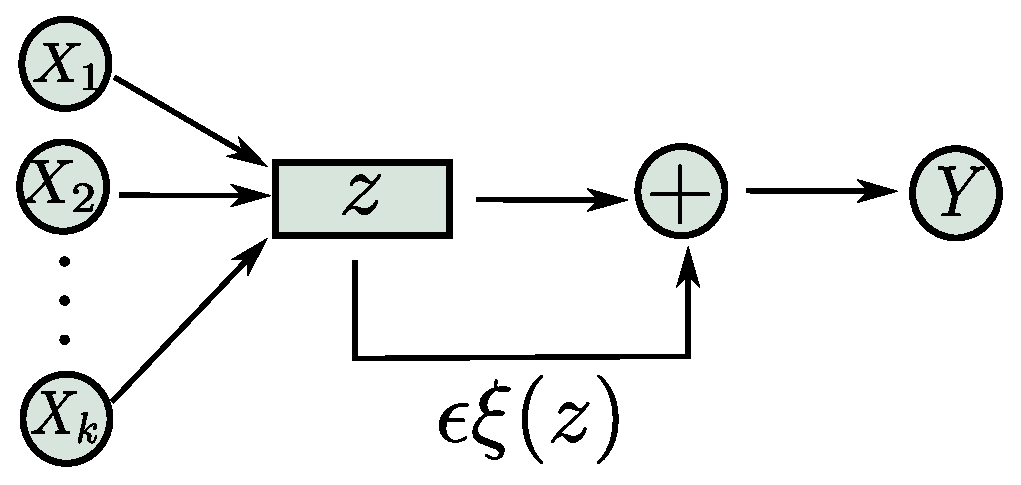
\includegraphics[width=\linewidth]{network_structure.eps}
\caption{The structure of one node neural network. The activation function $\sigma$ takes the form $\sigma(z)=z + \epsilon \xi(z)$}
\end{figure}

\section{Mathematical Model}\label{sec:mm}
We consider one node neural networks, whose structure is shown in Figure \ref{fig:ns}.
This type of network arises naturally from function approximation problems, where a target function $g$
is estimated by $\sigma(\sum_{i=1}^k w_i f_i)$ and the domain of definition for $f_i, g$ is a finite set.

To formulate the problem using neural networks, we consider a k dimensional random vector $\underline{X}=(X_1, \dots, X_k)$ and a random variable $Y$.
Our goal is to predict $Y$ using the neural network with $\underline{X}$ as input.
To be more specific, $Y$ is approximated by $ \sigma(\sum_{i=1}^k w_i X_i)$.
For a given problem, we have $n$ data pairs $(x_1, y_1), \dots, (x_n, y_n)$ and
the $\ell_2$ loss function is given by
$\ell_2(\underline{y}, \bm{x}) = \norm{\underline{y} - \sigma(\sum_{i=1}^k w_i \underline{x}_i)}^2 $
where $\underline{x}_i= (x_{1i}, \dots, x_{ni})^\T$ is the i-th column of the feature vector $\bm{x}$ and
$\underline{y} = (y_1, \dots, y_n)$ is the label vector. $\sigma$ is applied to a vector element-wise.
The optimal weight for a given activation function $\sigma$ is the solution to $\min \ell_2(\underline{y}, \bm{x})$.



For different problems, we suppose $\underline{y}, \bm{x}$ are drawing from some distribution $G$.
That is, we treat them as random vectors and rewrite them as $\underline{Y}, \bm{X}$.
We are interested to find a function $\sigma$ which minimizes
$\E[ \min \ell_2(\underline{Y}, \bm{X})]$.
Our constraint on the activation function $\sigma$ is that
$\sigma(z) = z + \epsilon \xi(z)$ where
$\epsilon$ is a small constant.
$\E[\xi(\bm{X}\underline{w})]=1$ where
$\bm{X}\underline{w} = \sum_{i=1}^k w_i \underline{X}_i$ is the matrix product with  $\underline{w}=(w_1, \dots, w_k)$.

We formulate universally good activation function $\sigma$ as follows:
\begin{definition}\label{def:ug}
Suppose $G$ is a distribution space for $(\bm{X}, \underline{Y})$,
$F$ is a function space for $\xi(z)$.
$\mathrm{E}[\sigma]$ is called the averaged estimation error whose definition is
\begin{align}\label{eq:ug}
\mathrm{E}(\sigma) = & \E[ \min_{\underline{w}} \norm{\underline{Y} - \sigma(\bm{X} \underline{w})}^2] 
%s.t. \,& \sigma(z) = z + \epsilon \xi(z) \nonumber \\
%&\E[\norm{\xi(\bm{X}\underline{w})}^2]=1
\end{align}
The function $\sigma^*$ which minimizes $\mathrm{E}(\sigma)$
is called the universally good activation function for the single node neural network.
\end{definition}

Definition \ref{def:ug} is a general formulation for any distribution space $G$.
To get some analytical result we should choose some specific distribution.
Indeed, we assume $\underline{Y}$ is Gaussian distribution with covariance matrix $\frac{1}{n} \mathbf{I}_n$ and
we choose $\bm{X}$ as uniformly distributed random orthogonal matrix \cite{eaton1989group}. The choice of $\bm{X}$ is based on the following observations: If each element of $\bm{X}'$ is iid N(0,1) random variables and $\sigma(\bm{X}'\underline{w}')$ is considered, we can make the transformation $\bm{X} = \bm{X}'(\bm{X}'^\T\bm{X}')^{-1/2}, \underline{w} = (\bm{X}'^\T\bm{X}')^{1/2}\underline{w}'$. We see that $\bm{X}'\underline{w}' = \bm{X}\underline{w}$. From \cite[Proposition 7.1]{eaton1989group} $\bm{X}$ is random orthogonal matrix.
Further we assume $\underline{Y}$ and $\bm{X}$ are independent.
This defines our distribution space $G$. Such choice is natural and it leads to simple expression of the averaged error for linear function.

\begin{proposition}\label{prop:linear}
Let $\sigma_0$ be the identity function. That is $\sigma_0(z) = z$. Then $\mathrm{E}(\sigma_0) = 1 - \frac{k}{n}$.\end{proposition}

Proposition \ref{prop:linear} says the averaged estimation error $\mathrm{E}$ for linear function is equal to $1-\frac{k}{n}$.
This result is consistent with our intuition
since we use $k$ degrees of freedom to estimate arbitrary vector in $n$ dimensional space.

The proof of Proposition \ref{prop:linear} depends on the following lemma:
\begin{lemma}\label{lem:A}
Suppose $\bm{X}$ is uniformly distributed random orthogonal matrix, $\bm{A} = \bm{X}\bm{X}^\T$.
Then $\E[\bm{A}] = \frac{k}{n} \mathbf{I}_n$.
\end{lemma}
We defined random matrix $\bm{A}$ in Lemma \ref{lem:A} for notation convenience.
Since $\bm{X}$ is orthogonal, $\bm{A}$ is idempotent. That is, we have $\bm{A}^2 = \bm{A}$.

We have analyzed the averaged error for linear function. To extend our result on general non-linear functions, we need to choose a proper function space $F$. By detailed analysis we consider a "local" regime. That is, differential functions which are "near" to linear function. The distance is quantified by a positive value $\epsilon$. Thus we consider $F_{\sigma_0}(\epsilon) =\{ \sigma \,|\, \norm{\sigma - \sigma_0} \leq \epsilon\}$. Then all differential functions can be treated as $\cup_{\epsilon>0} F(\epsilon)$. The norm is actually the expectation w.r.t. the distribution space $G$. That is $\E[\norm{(\sigma - \sigma_0)(\bm{A}\underline{Y})}^2] \leq \epsilon^2$.

We are particularly interested in how the averaged error changes when $\sigma$ is contracted to $\sigma_0$ along a certain path in $F(\sigma)$. That is, given a function $\xi$ we can construct $\sigma = \sigma_0 + \epsilon \xi$ where $\xi \in F_0 = \{\xi | \norm{\xi} \leq 1 \}$. $\sigma \to \sigma_0$ is equivalent to $\epsilon \to 0$.

To measure the change rate of $E[\sigma]$ in local regime of linear function we introduce the concept of the index of averaged estimation error as follows:
\begin{definition}
Let $\xi \in F_0$, the index of averaged estimation error for $\xi$ is
\begin{equation}\label{eq:Cxi}
\mathrm{C}[\xi] = \lim_{\substack{\epsilon \to 0 \\ \sigma = \sigma_0 + \epsilon \xi}} \frac{E[\sigma] - E[\sigma_0]}{\epsilon^2}
\end{equation}
\end{definition}

$\mathrm{C}[\xi]$ can represent the change rate of perturbation from linear function. If $\mathrm{C}[\xi]$ is negative for a given $\xi$, we can decrease $\mathrm{E}[\sigma]$ in the rate of $\abs{\mathrm{C}[\xi]}$ along  the perturbation path of $\xi$.
The definition of $\mathcal{C}[\xi]$ in Equation \eqref{eq:Cxi} can also be rewritten in another way as
$\mathrm{E}[\sigma] = \mathrm{E}[\sigma_0] +
\mathrm{C}[\xi]\epsilon^2 + o(\epsilon^2)$. In this form, we can see more clearly that $\mathrm{C}[\xi]$ is the coefficient of second order term of $\mathrm{E}[\sigma]$.

To justify the definition of $\mathrm{C}[\xi]$, we need to show the limit in Equation \eqref{eq:Cxi} exists, which is guaranteed by the following proposition:
%For functional space $F$, we choose $P_m(z)$,
%which consists of polynomials with the highest degree no more than $m$.

\begin{proposition}\label{prop:Esigma} 
Let $\nabla \xi(\underline{z})  = \diag[\xi'(\underline{z}_1), \dots, \xi'(\underline{z}_n)]$, we have
\begin{align}\notag
\mathrm{C}[\xi]= & \E[\norm{\xi(\bm{A}\underline{Y})}^2 -
\norm{\bm{X}^\T\xi(\bm{A}\underline{Y})}^2 \\
&- \norm{\bm{X}^\T \nabla\xi(\bm{A}\underline{Y})(Y-\bm{A}\underline{Y})}^2]
\end{align}
\end{proposition}

Our goal is to get the largest decreasing rate for $E[\sigma]$ from $E[\sigma_0]$, this is equivalent to solve an optimization problem $\min \mathrm{C}[\xi]$ constraint by $\xi \in F_0$. It is hard to optimize on $F_0$ directly and we consider $F_{0,m} = F_0 \cap P_m$ first. $P_m$ consists of polynomials with the highest degree no more than $m$. And we have $F_0 = \lim_{m\to \infty} F_{0,m}$.

For $\xi \in F_{0,m}$ we have the following result:
\begin{proposition}\label{prop:quadratic}
If
$\xi(z) = \sum_{i=0}^m \underline{q}_i z^i$,
and $m \ll k$, then we have 
\begin{align}
\mathrm{C}[\xi] &= (1-\frac{k}{n}) \underline{p}^\T \mathbf{M} \underline{p} \notag\\
\textrm{where }\underline{p}_i &= \frac{k^{i/2}}{n^{- 1/2 + i}}\underline{q}_i\label{eq:pqt} \\
\mathbf{M}_{ij} =& -\delta(i,j)(i-1)(j-1)(i+j-3)!! \notag
\end{align}
The constraint $\xi \in F_{0,m}$ is equivalent with
\begin{align}
\underline{p}^\T \mathbf{N} \underline{p} & = 1 \notag\\
\mathbf{N}_{ij}  & = \delta(i,j)(i+j-1)!!
\end{align}
\end{proposition}

Proposition \ref{prop:quadratic} gives a feasible approach to choose the optimal $\xi$ by solving a quadratic optimization problem. We make the assumption $
m << k$ to write $M_{ij}$ in a concise form. This assumption requires that we should choose low degree polynomials as activation function and the number of node $k$ should be relatively large to represent features. Since computational cost
is proportional to the degree of polynomials, our assumption does not lose practicality. 

\section{Hermite Polynomials}\label{sec:hp}

One of our major result is that we find Proposition \ref{prop:quadratic} leads naturally to the Hermite Polynomials solutions. Probabilists' Hermite polynomial $H_m(x) (m=1,2,\dots)$ is a serial of polynomial with the orthogonal property $ \E[H_m(X)H_n(X)] = n! \delta_{mn}$ where $X$ is standard normal random variable.
The highest degree of $H_m(x)$ is $m$. $\xi(z) \in F_{0, m}$ which minimizes $\mathrm{C}[\xi]$ has the following relationship with Hermite polynomials:
\begin{proposition}\label{prop:value}
Let
\begin{equation}\label{eq:ximopt}
    \xi_m(z) = \frac{1}{\sqrt{m!n}} H_m(\frac{n}{k^{1/2}} z)
\end{equation}
Then $\mathrm{C}[\xi_m] = -(1-\frac{k}{n})(m-1) \leq \mathrm{C}[\xi] $ for all $\xi \in F_{0, m}$.
\end{proposition}
Proposition \ref{prop:value} also gives the lower bound for $\mathrm{C}[\xi]$.
It says the local decreasing rate of $\mathrm{E}[\sigma]$ is strictly linearly improved if we increase the degree of Hermite polynomials. This result is made under the assumption $ m << k$ and in general case when $ m << k$ does not hold, we find by experiments that $-(1-\frac{k}{n})(m-1) < \mathrm{C}[\xi]$ while $\mathrm{C}[\xi]$ decreases in linear way.

%\section{Experiment Result}\label{sec:er}

%To verify the change rate of the index of averaged estimation error $C[\xi]$ as we increase the maximal degree of polynomials $m$, we conduct a simple %experiment. We choose $n=180, k=120$ and use $\xi_m(z)$ from Proposition
%\ref{prop:value}, normalized polynomials with only highest degree $\frac{(nz/\sqrt{k})^m}{\sqrt{(2m-1)!!n}}$ as activation function. Using the Monte Carlo method to compute $\mathrm{C}[\xi]$ from Proposition \ref{prop:Esigma}, the result is shown in Figure \ref{fig:fixednk}. As can be seen, the Hermite polynomial results coincide with the theoretical lower bound in Proposition \ref{prop:value}; For other polynomials, it cannot achieve the minimum value but we can still see that the nearly linear relationship between $C[\xi]$ and degree $m$.

%\begin{figure}
%    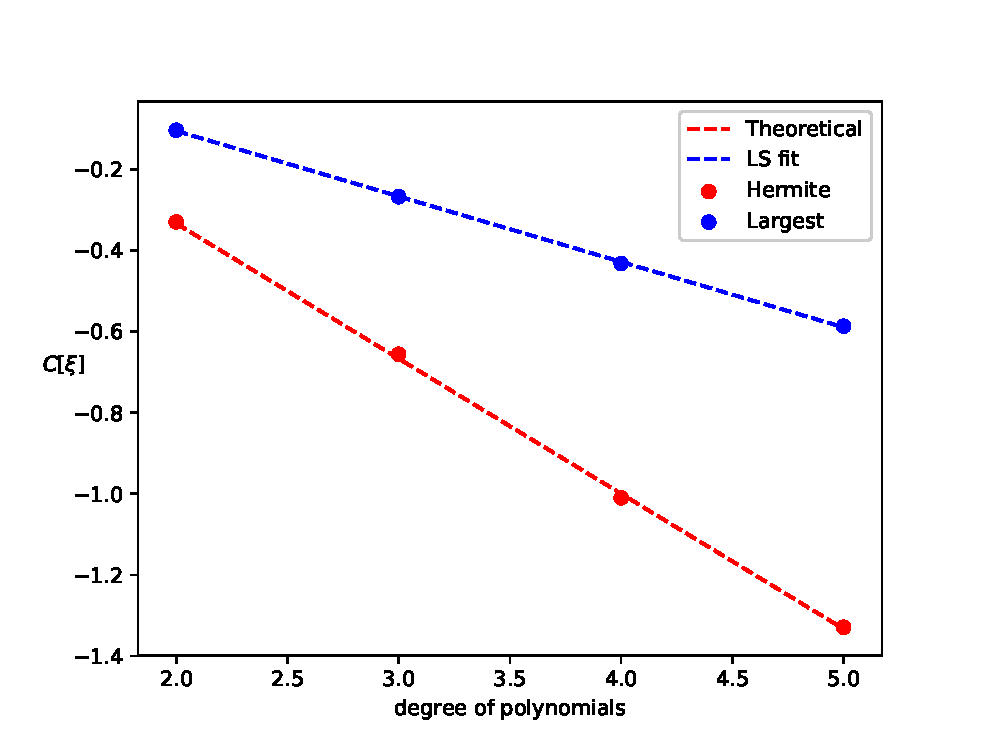
\includegraphics[width=\linewidth]{fixed_nk.eps}
%    \caption{Illustration of the linear decreasing property of $C[\xi]$}\label{fig:fixednk}
%\end{figure}


\section{Conclusion}\label{sec:con}

In this paper, we investigate the mechanism of non-linearity in one node neural network. It can decrease the loss linearly as we increase the maximal degree if we consider a small polynomial perturbation of linear activation function. How non-linearity works in more complex neural networks will be considered in our future work. 

%\section*{Acknowledgment}
\appendix
\begin{proof}[Proof of Lemma \ref{lem:A} ]
By the symmetric property we only need to show $\E[\bm{A}_{11}] = \frac{k}{n}$ and
$\E[\bm{A}_{12}] = 0$. For the first equation, we have $n\E[\bm{A}_{11}]
= \sum_{i=1}^n \E[\bm{A}_{ii}] = \sum_{i=1}^n \E[ \sum_{j=1}^k \bm{X}^2_{ij}] =
\sum_{j=1}^k \E[\sum_{i=1}^n \bm{X}^2_{ij}]$. Since the norm of $\bm{X}_j$ is 1,
the whole summation evaluates to $k$. Therefore $\E[\bm{A}_{11}] = \frac{k}{n}$.

On the other hand, $\bm{X}$ can be treated as an $n\times k$ subblock of an $n\times n$
random orthogonal matrix $\bm{\bar{X}}$ with the property that $\bm{X}_{ij} = \bm{\bar{X}}_{ij}$
for $j\leq k$. For $\bm{\bar{X}}$, the first and second row are orthogonal:
 $\E[\sum_{j=1}^n \bm{\bar{X}}_{1j}\bm{\bar{X}}_{2j}] = 0 $ which leads to
 $\E[\bm{X}_{1j}\bm{X}_{2j}] = 0$ for $j \leq k$. Hence $\E[\bm{A}_{12}]=
 \E[\sum_{j=1}^k \bm{X}_{1j}\bm{X}_{2j}]=0$.
\end{proof}
\begin{proof}[Proof of Proposition \ref{prop:linear}]
    When $\epsilon = 0$, the optimal $\underline{w}_0 = \bm{X}^\T\underline{Y}$. Therefore
    $\E[\norm{\underline{Y} - \sigma(\bm{X} \underline{w}_0)}^2] = \E[\norm{\underline{Y}-\bm{X}\bm{X}^\T\underline{Y}}^2]$
    The expectation can be taken by $\underline{Y}$ first and then by $\bm{X}$.
    Let $\underline{Z} = (I-\bm{A}) \underline{Y}$ which transforms a Gaussian random vector $\underline{Y}$.
    for given $\bm{X}$. Therefore $\E_{\underline{Y}}[\norm{\underline{Z}}^2] = \Tr[(I-A)^\T\Cov[Y](I-A)]
    = \frac{1}{n}\Tr[I - A]$. Using Lemma \ref{lem:A}. $\mathrm{E}(\sigma) = 1 - \frac{k}{n}$ follows.
\end{proof}
\begin{proof}[Proof of Proposition \ref{prop:Esigma} ]
For the problem $\min_{\underline{w}} \norm{\underline{Y} - \sigma(\bm{X} \underline{w})}$
with $\sigma = \sigma_0 + \epsilon \xi$. We can write $\underline{w} = \underline{w}_0
+ \epsilon \underline{\hat{w}} + o(\epsilon)$ where $\underline{w}_0 = \bm{X}^\T \underline{Y}$ is the minimizer for
$\epsilon = 0$. That is, we assume $\underline{w}$ can be expanded near $\underline{w}_0$
using $\epsilon$ terms. We can expand $\norm{\underline{Y} - \sigma(\bm{X} \underline{w})}$ 
up to $o(\epsilon^2)$ as
\begin{align*}
&\norm{\underline{Y} - \bm{X} \underline{w}_0 - \epsilon \bm{X} \underline{\hat{w}} -
\epsilon^2 \bm{X} \underline{\tilde{w}} - \epsilon \xi(\bm{X} \underline{w}_0 +
\epsilon \bm{X} \underline{\hat{w}}) }^2 \\
= & \norm{ \underline{Y} - \bm{X}  \underline{w}_0 -
\epsilon (\bm{X}\underline{\hat{w}} + \xi(\bm{X} \underline{w}_0 )) \\
&-  \epsilon^2(\bm{X}\underline{\tilde{w}} + \nabla \xi(\bm{X} \underline{w}_0 )\bm{X}\underline{\hat{w}})}^2 \\
= & \norm{\underline{Y}-\bm{X} \underline{w}_0  }^2 -
2 \epsilon (\bm{X} \underline{\hat{w}} +
\xi(\bm{X} \underline{w}_0))^\T (\underline{Y} - \bm{X} \underline{w}_0) +\\
& +  \epsilon^2(\norm{\bm{X}\underline{\hat{w}} + \xi(\bm{X} \underline{w}_0)}^2 \\
& -
2 (\bm{X} \underline{\tilde{w}}+
\nabla \xi(\bm{X} \underline{w}_0)\bm{X}\underline{\hat{w}})^\T(\underline{Y}-\bm{X} \underline{w}_0))
\end{align*}
$\bm{X}\underline{w}_0 = \bm{X}\bm{X}^\T \underline{Y}$ is the projection of $\underline{Y}$ onto linear subspace spanned by
columns of $\bm{X}$.

We first show that in the expansion of $\E[\sigma]$, the coefficient of $\epsilon$ is zero.
We use $\tilde{\underline{Y}}$ to denote the mirror of $\underline{Y}$ about this linear subspace.
Then we have
$\bm{X}\bm{X}^\T \underline{Y} = \bm{X}\bm{X}^\T \tilde{\underline{Y}}$ and
$(\underline{Y}- \bm{X}\bm{X}^\T\underline{Y}) = -(\tilde{\underline{Y}} - \bm{X}\bm{X}^\T \tilde{\underline{Y}})$.
This symmetric property leads to $\E_{\underline{Y}}[\xi(\bm{X}\underline{w}_0)^\T (\underline{Y}-\bm{X}\underline{w}_0)]=0$.
On the other hand, since $\bm{X}^\T \bm{X} = \mathbf{I}_k$. $(\bm{X}\underline{\hat{w}})^\T (\underline{Y}-\bm{X}\underline{w}_0) = \underline{\hat{w}}^\T (X^\T \underline{Y} - \underline{w}_0) = 0$.

Next, we minimize the coefficient of $\epsilon^2$ by $\underline{\hat{w}}$, which simplifies to 
\begin{equation}\label{eq:st}
\norm{\bm{X}\underline{\hat{w}} + \xi(\bm{X} \underline{w}_0)}^2-
2 (
\nabla \xi(\bm{X} \underline{w}_0)\bm{X}\underline{\hat{w}})^\T(\underline{Y}-\bm{X} \underline{w}_0)
\end{equation}
due to $(\bm{X}\underline{\tilde{w}})^\T (\underline{Y}-\bm{X}\underline{w}_0) = 0 $.
The expression in \eqref{eq:st} is quadratic about $\underline{\hat{w}}$. The minimum value is achieved  at
$$
\underline{\hat{w}} =  \bm{X}^\T(\nabla\xi(\bm{X}\bm{X}^\T \underline{Y})
(\underline{Y}-\bm{X}\bm{X}^\T \underline{Y}) - \xi(\bm{X}\bm{X}^\T \underline{Y}))
$$
Substituting $\underline{\hat{w}}$ in expression in \eqref{eq:st} with the above equation we can get the minimum value for the coefficient of $\epsilon^2$, which is exactly $C[\xi]$.
\begin{align*}
C[\xi] = & \E[\norm{\xi(\bm{X}\bm{X}^\T\underline{Y})}^2 -
\norm{\bm{X}^\T\xi(\bm{X}\bm{X}^\T\underline{Y})}^2 \\
& -
\norm{\bm{X}^\T \nabla\xi(\bm{X}\bm{X}^\T\underline{Y})(\underline{Y}-\bm{X}\bm{X}^\T\underline{Y})}^2]
\end{align*}
\end{proof}
\begin{lemma}\label{lemma:Isserlis2}
     Suppose $(X,Y)$ is two-dimensional Gaussian vector,
     has zero mean and covariance vector $\Sigma$, $ i + j $ is even, then we have
\begin{equation*}
    \E[X^i Y^j] =
    \sum_{k=0}^{\min\{i,j\}}
    \frac{\delta(k, i) i! j!}{k! (i-k)!!(j-k)!!}
    \Sigma_{12}^k \Sigma_{11}^{(i-k)/2}\Sigma_{22}^{(j-k)/2}
\end{equation*}
\end{lemma}
\begin{proof}
Using Isserlis' theorem \cite{isserlis1918formula} we obtain
$  \E[X^i Y^j] = \sum_{k=0}^{\min\{i,j\}} C_k \Sigma_{12}^k \Sigma_{11}^{(i-k)/2}\Sigma_{22}^{(j-k)/2}$. Since the power of $\Sigma_{11}$ should be an integer, $C_k = 0$ if $\delta(k, i) = 0$. If $\delta(k, i) = 1$, we choose $k$ items of $X$ and $Y$ to form $\Sigma_{12} = \E[XY]$, which has $\binom{i}{k}\binom{j}{k}$ choices. For the remaining $(i-k)$ number of $X$, we should pair them, which has $\frac{1}{(\frac{i-k}{2})!}\prod_{i=1}^{(i-k)/2} \binom{2i}{2} = \frac{(i-k)!}{(i-k)!!}$ number of choices; For $(j-k)$ number of $Y$, it is $\frac{(j-k)!}{(j-k)!!}$; Finally, for $k$ pairs of $XY$, we have $k!$ number of choices. The product $\binom{i}{k}\binom{j}{k}\frac{(i-k)!}{(i-k)!!}\frac{(j-k)!}{(j-k)!!}k!$ is the coefficient $C_k$.
\end{proof}
%\begin{lemma}\label{lemma:A1112}
%For random matrix $\bm{A}$ we have $\E[\bm{A}_{11}^t] = \prod_{i=0}^{t-1} \frac{k+2t}{n+2t}$ and
%$\E[\bm{A}_{12}^2] = \frac{(n-k)k}{(n-1)n(n+2)}$.
%\end{lemma}
%\begin{proof}[Proof of Lemma \ref{lemma:A1112}]
%Then the high order moment of $\bm{A}_{11}^t$ follows from \cite[Eq. 8]{weisstein}. To compute $\E[\bm{A}_{12}^2]$, using the symmetric property first we %have $\E[\bm{A}_{11}^2] = k\E[\bm{X}_{11}^4] + k(k-1)\E[\bm{X}_{11}^2 \bm{X}_{12}^2] \Rightarrow
%\frac{k(k+2)}{n(n+2)} = \frac{3k}{n(n+2)} + (k-1) (k \E[\bm{X}_{11}^2 \bm{X}_{12}^2])$.
%Also $\E[\bm{A}_{12}^2] = \E[(\sum_{i=1}^k \bm{X}_{11} \bm{X}_{12})^2]
%= k \E[\bm{X}_{11}^2\bm{X}_{12}^2] + k(k-1)\E[\bm{X}_{11}\bm{X}_{12}\bm{X}_{21}\bm{X}_{22}]
%$.
%Since $\sum_{i=1}^n \bm{X}_{1i} \bm{X}_{2i} = 0$, multiplying this equation by $\bm{X}_{12}\bm{X}_{22}$ and taking the expectation
%we have $\E[\bm{X}_{11}\bm{X}_{12}\bm{X}_{21}\bm{X}_{22}] = \frac{-1}{n-1} \E[\bm{X}^2_{11}\bm{X}^2_{12}]$.

%Therefore $\E[\bm{A}^2_{12}]=(1-\frac{k-1}{n-1}) \frac{k}{n(n+2)}$.
%\end{proof}
\begin{lemma}\label{lemma:UUN}
    \begin{equation}\label{eq:UUN}
        \delta(i, j) (i+j-1)!! = \sum_{k=0}^{\min\{i, j\}}
        \delta(k, i) \delta(k, j) \frac{i! j!}{(i-k)!!(j-k)!! k!}
    \end{equation}
\end{lemma}
\begin{proof}[Proof of Lemma \ref{lemma:UUN} ]
    If $ i + j $ is odd, $ \delta(i, j) = 0 $ and
    $ \delta(k, i)\delta(k, j) = 0 $. Then Equation \eqref{eq:UUN} holds.
    Therefore we only need to consider the case if $ i + j $ is even.
    First we define $A(i, j) = \sum_{k=0}^{\min\{i, j\}}
    \delta(k, i) \delta(k, j) \frac{i! j!}{(i-k)!!(j-k)!! k!}$.
    Then we have
    \begin{align}
        & A(2i+1, 2j+1) = \sum_{k=0}^{\min\{i,j\}}
        \frac{(2i+1)!(2j+1)!}{(2i-2k)!!(2j-2k)!!(2k+1)!} \notag\\
        &= \sum_{k=0}^{\min\{i,j\}}
        \frac{(2i+1)!(2j)!\left(\frac{1}{2j-2k} + \frac{1}{2k+1}\right)}{(2i-2k)!!(2j-2k-2)!!(2k)!}
        \notag\\
        &= (2i + 1) A(2i, 2j) + (2j) A(2i+1, 2j-1) \label{eq:Bij}
    \end{align}
    The above formula holds for $ i \leq j-1 $ because of choice of $\min\{i,j\}$.
    We can use the symmetric property $A(i,j)=A(j,i)$
    to show Equation \eqref{eq:Bij} also holds for $ i \geq j $.
    Similarly we have
    \begin{equation}\label{eq:Aij}
        A(2i, 2j) = (2j - 1) A(2i, 2j-2) + (2i) A(2i-1, 2j-1)
    \end{equation}
    From Equation (\ref{eq:Bij}, \ref{eq:Aij}), we can use mathematical induction to show
  \begin{align*}
       A(2i, 2j)  &= (2i + 2j - 1)!! \\
     A(2i+1, 2j+1) &= (2i + 2j + 1)!!
  \end{align*}
    Therefore $A(i,j) = (i+j-1)!!$ if $i + j $ is even.
    Based on our discussion on the parity of $i+j$, in general we have $A(i,j)=\delta(i,j)(i+j-1)!!$
    which proves Lemma \ref{lemma:UUN}.
\end{proof}
\begin{lemma}\label{lemma:UUM}
    \begin{align}
        &\delta(i, j)(i-1)(j-1)(i+j-3)!!  \notag\\
        =&\sum_{k=0}^{\min\{i, j\}}
        \delta(k, i) \delta(k, j) \frac{(k-1)i!j!}{(i-k)!!(j-k)!!k!}
    \end{align}
\end{lemma}
\begin{proof}
    Using results from Lemma \ref{lemma:UUN},
    \begin{align*}
        & \textrm{RHS}  = \sum_{k=1}^{\min\{i, j\}}
        \delta(k, i) \delta(k, j) \frac{i!j!}{(i-k)!!(j-k)!!(k-1)!}\\
        & -\sum_{k=0}^{\min\{i, j\}}
        \delta(k, i) \delta(k, j) \frac{i!j!}{(i-k)!!(j-k)!!k!}  \\
        & =  ij\sum_{k=0}^{\min\{i-1, j-1\}}
        \delta(k, i) \delta(k, j) \frac{(i-1)!(j-1)!}{(i-1-k)!!(j-1-k)!!k!} \\
        & -\delta(i, j)(i+j-1)!! \\
        & = \delta(i, j)ij(i+j-3)!! - \delta(i, j)(i+j-1)!! \\
        & = \delta(i, j)(i-1)(j-1)(i+j-3)!!
    \end{align*}
\end{proof}
\begin{proof}[Proof of Proposition \ref{prop:quadratic}]
Let $\underline{Z} = \bm{A}\underline{Y}, \underline{Z'} = (\mathbf{I} - \bm{A})\underline{Y}$. Given $\bm{X}$, $\underline{Z}$ is Gaussian vector with covariance matrix $\bm{A} \Cov[\underline{Y}] \bm{A}^\T = \frac{\bm{A}}{n}$. Similarly, $\Cov[\underline{Z'}] = \frac{\mathbf{I} - \bm{A}}{n}$. Using $\bm{A}^2 = \bm{A}$ we have $\E[\underline{Z'}\underline{Z}^\T] = 0$. That is, $\underline{Z'}$ and $\underline{Z}$ are independent. The expectation of $\E[f(\underline{Z}_i)g(\underline{Z'}_j)] = \E[f(\underline{Z}_i)]\E[g(\underline{Z'}_j)]$ for arbitrary function.
    
Let $\mathbf{C}_1 = \E_{\underline{Y}} [\norm{\xi(\bm{A}\underline{Y})}^2]$, $\mathbf{C}_2 
= \E_{\underline{Y}}
[\norm{\bm{X}^\T\xi(\bm{A}\underline{Y})}^2]$, $\mathbf{C}_3 
= \E_{\underline{Y}}
[\norm{\bm{X}^\T \nabla\xi(\bm{A}\underline{Y})(Y-\bm{A}\underline{Y})}^2]$,
$\mathrm{C}[\bm{X}, \xi] :=  \mathrm{C}_1 - \mathrm{C}_2 - \mathrm{C}_3$, Then $\mathrm{C}[\xi] = \E_{\bm{X}}[\mathrm{C}[\bm{X}, \xi]]$.
We then have
\begin{align*}
    \mathrm{C}_1 &=\E[\norm{\xi(\underline{Z})}^2] = \sum_{i=1}^n \E_{Z|X}[\xi^2(\underline{Z}_i)] \\
    \mathrm{C}_2 &= \sum_{i,j=1, i \neq j}^n \bm{\bm{A}}_{ij}\E[\xi(\underline{Z}_i)\xi(\underline{Z}_j)] +
    \sum_{i=1}^n \bm{\bm{A}}_{ii}  \E[\xi^2(\underline{Z}_i)] \\
    \mathrm{C}_3 & = \sum_{i,j=1, i \neq j}^n \bm{A}_{ij}\bm{\Sigma}_{ij} +
    \sum_{i=1}^n \bm{A}_{ii}\bm{\Sigma}_{ii}    \\
    \bm{\Sigma}_{ii} &=  \E[ [\underline{Z'}_i]^2 [\xi'(\underline{Z}_i)]^2] = \frac{1-\bm{A}_{ii}}{n}[\xi'(\underline{Z}_i)]^2   \\
    \bm{\Sigma}_{ij} &=  \E[\underline{Z'}_i \underline{Z'}_j \xi'(\underline{Z}_i)
    \xi'(\underline{Z}_j)]
     = - \frac{\bm{A}_{ij}}{n} \E[ \xi'(\underline{Z}_i)
    \xi'(\underline{Z}_j)]
\end{align*}
The expression for $\Sigma_{ij}$ holds for $i \neq j$ above. Combining the above equations we have
\begin{align*}
   &  \mathrm{C}[\bm{X}, \xi] = \sum_{i=1}^n (1-\bm{A}_{ii})(\E[\xi^2(\underline{Z}_i)] -
    \frac{ \bm{A}_{ii}}{n} \E[ \xi'^2(\underline{Z}_i)]) \\
    &- \sum_{i,j=1, i \neq j}^n \bm{A}_{ij} (\E[\xi(\underline{Z}_i)\xi(\underline{Z}_j)] -
    \frac{\bm{A}_{ij}}{n}\E[\xi'(\underline{Z}_i) \xi'(\underline{Z}_j)])
\end{align*}
By symmetric property, we can simplify the above equation as:
\begin{align*}
    &  \mathrm{C}[\bm{X}, \xi] =n(1-\bm{A}_{11})(\E[\xi^2(\underline{Z}_1)] -
    \frac{\bm{A}_{11}}{n}  \E[ \xi'^2(\underline{Z}_1)]) \\
    &- n(n-1)\bm{A}_{12}(\E[\xi(\underline{Z}_1)\xi(\underline{Z}_2)] -
    \frac{\bm{A}_{12}}{n}\E[\xi'(\underline{Z}_1)
   \xi'(\underline{Z}_2)])\nonumber
\end{align*}

Since 
$\xi(z) = \sum_{i=0}^m \underline{q}_i z^i $,
there will be an $(m+1) \times (m+1) $ random matrix $\bm{M}$ and
we can write $\mathrm{C}[\bm{X}, \xi]$
as the quadratic form $ \underline{q}^T \bm{M} \underline{q} $.
The element $\bm{M}_{ij}$ is the coefficient of $a_ia_j$:
\begin{align*}
    \bm{M}_{ij} &= n(1-\bm{A}_{11}) (\E[\underline{Z}_1^{i+j}] -
    ij \frac{1}{n}\bm{A}_{11} \E[\underline{Z}_1^{i+j-2}])  \\
    &-n(n-1)\bm{A}_{12}(\E[\underline{Z}_1^i \underline{Z}_2^j] - ij \frac{1}{n}\bm{A}_{12}\E[\underline{Z}_1^{i-1}\underline{Z}_2^{j-1}])
\end{align*}
Since $\bm{Z}_1$ is Gaussian, $\E[Z_1^{2t}] = \frac{1}{n^t}\bm{A}_{11}^t (2t-1)!!$. If $\delta(i, j) = 0, \bm{M}_{ij}=0$. Otherwise,
let $ 2t = i + j $, from Lemma \ref{lemma:Isserlis2}, $\E[\underline{Z}_1^i \underline{Z}_2^j]$ can be expanded and we have:
\begin{align*}
    &\bm{M}_{ij} = -n(1-\bm{A}_{11}) \frac{\bm{A}_{11}^t}{n^t}(i-1)(j-1)(2t-3)!! \\
    &-\frac{n(n-1)\bm{A}_{12}}{n^t}\sum_{s=0}^{\min\{i,j\}}
    \frac{\delta(s,i)(1-s)i!j!}{s!(i-s)!!(j-s)!!}
    \bm{A}_{12}^s \bm{A}_{11}^{\frac{i - s}{2}}\bm{A}_{22}^{\frac{j - s}{2}}
\end{align*}
$C[\xi] = \E_{\bm{X}}[\mathrm{C}[\bm{X}, \xi]] =  \underline{q}^T \mathbf{M}' \underline{q}$ where $\mathbf{M}'_{ij} = \E_{\bm{X}} [\bm{M}_{ij}] = -M_1 + M_2$
where 
\begin{align*}
    M_1 & =   \frac{\E[\bm{A}_{11}^t]-\E[\bm{A}_{11}^{t+1}]}{n^{t-1}}(i-1)(j-1)(2t-3)!! \\
    M_2 & = \frac{n-1}{n^{t-1}}\sum_{s=0}^{\min\{i,j\}}
    \frac{\delta(s,i)(s-1)i!j!}{s!(i-s)!!(j-s)!!}
    \E[\bm{A}_{12}^{s+1} \bm{A}_{11}^{\frac{i - s}{2}}\bm{A}_{22}^{\frac{j - s}{2}}]
\end{align*}
We estimate the order of positive number $M_1, M_2$ under the condition $ m << k$. Since $k$ is large, we assume $k, n \to +\infty$ while $m$ is finite. Let $ r= \frac{k}{n}$. Since $\bm{A}=\bm{X}\bm{X}^\T$, from Proposition 7.2, Chapter 7 of \cite{eaton1989group} we can get $\bm{A}_{11}$ is Beta distribution with parameter $B(\frac{k}{2}, \frac{n-k}{2})$.
From Theorem 1 of \cite{multivariateBeta},
$\E[\bm{A}_{11}^t]-\E[\bm{A}_{11}^{t+1}] = (1-r)\prod_{s=0}^{t-1} \frac{2s+k}{2s+n+2} \sim (1-r)r^t$. Therefore $M_1 \sim \frac{(1-r)r^t}{n^{t-1}}(i-1)(j-1)(2t-3)!!$.
We consider $s+1$ is even, $\E[\bm{A}_{12}^{s+1} \bm{A}_{11}^{\frac{i - s}{2}}\bm{A}_{22}^{\frac{j - s}{2}}] \leq \sqrt{\E[\bm{A}_{12}^{s+1}\bm{A}_{11}^{i-s}]\E[\bm{A}_{12}^{s+1}\bm{A}_{22}^{j-s}]}$. When $k, n$ are sufficiently large, we can treat $\bm{A}_{11}, \bm{A}_{12}$ as joint Gaussian. From Theorem 2 of \cite{multivariateBeta}: $\E[\bm{A}_{12}^{s+1}\bm{A}_{11}^{i-s}] \sim s!! r^{i-s}(\frac{r(1-r)}{n})^{(s+1)/2}$. Similarly $\E[\bm{A}_{12}^{s+1}\bm{A}_{22}^{j-s}] \sim s!! r^{j-s}(\frac{r(1-r)}{n})^{(s+1)/2}$. It implies that $\E[\bm{A}_{12}^{s+1} \bm{A}_{11}^{\frac{i - s}{2}}\bm{A}_{22}^{\frac{j - s}{2}}] \leq (s!!) r^{t-s}(\frac{r(1-r)}{n})^{(s+1)/2} \leq r(1-r)$. We can get an upper bound of $M_2$ using Lemma \ref{lemma:UUM}: $M_2 \leq \frac{1}{n^{t-2}} (i-1)(j-1)(2t-3)!!\E[\bm{A}_{12}^{4} \bm{A}_{11}^{\frac{i - 3}{2}}\bm{A}_{22}^{\frac{j - 3}{2}}] \leq \frac{(1-r)^2 r^{t-1}}{n^t}3(i-1)(j-1)(2t-3)!!= \frac{3(1-r)}{k} M_1$.
When $k \to \infty$, we see that $M_2$ can be ignored and $\mathbf{M}'_{ij} = -\delta(i,j)\frac{(1-r)r^t}{n^{t-1}}(i-1)(j-1)(2t-3)!!$. By changing of variables by Equation \ref{eq:pqt} we can get the correspondence $\mathbf{M}_{ij} = \frac{n^{-1+2t}}{k^t} \mathbf{M}'_{ij} = -\delta(i,j)(1-r)(i-1)(j-1)(2t-3)!!$. 

To get the constraint on $\underline{q}$, we should choose $\norm{\xi} = 1$, which is equivalent to $\E_{\bm{X}}[\mathrm{C}_1] = 1$. By some computation we can get the expression of $\mathrm{N}$ when $ m << k$.

\end{proof}

\begin{lemma}\label{lemma:Upem}
Let $\mathbf{U}$ be an $(m+1) \times (m+1)$ upper triangular matrix defined by
$U_{ij} = \delta(i, j) \frac{j!}{(j-i)!!\sqrt{i!}} \textrm{ for } 0 \leq i\leq j \leq m$, $\underline{e_m}$ is an $(m+1)$ dimensional vector whose elements are zero except that the last element is 1. $\underline{p}_i = \delta(i, m) (-1)^{(m-i)/2}\frac{\sqrt{m!}}{i!(m-i)!!}$.
Then we have $ \mathbf{U} \underline{p} = \underline{e_m}$.
\end{lemma}
\begin{proof}[Proof of Lemma \ref{lemma:Upem} ]
    For $ i = m, \mathbf{U}_{mm} = \sqrt{m!}$, we can show that $\mathbf{U}_{mm} \underline{p}_m = 1 $; For $ 0\leq i < m $ we
    will show that $ \sum_{j=i}^m \mathbf{U}_{ij} \underline{p}_j = 0 $. In specific form as
    \begin{equation}\label{eq:jimf}
    \sum_{j=i}^m \delta(i, j) \frac{j!}{(j-i)!!\sqrt{i!}}  \frac{\delta(j, m)(-1)^{(m-j)/2}\sqrt{m!}}{j!(m-j)!!} = 0
    \end{equation}
    If $ \delta(i, m) = 0$, $\delta(i, j)\delta(j, m) = 0$ and Equation \eqref{eq:jimf} holds. Otherwise let $2m' = m - i$,    
    Equation \eqref{eq:jimf} is equivalent to
    $ \displaystyle\sum_{j=i, \delta(i,j)=1}^m  \frac{(-1)^{(m-j)/2}}{(m-j)!!(j-i)!!}  = 0  \iff  $
    $\displaystyle\sum_{j=0, j \textrm{ is even}}^{2m'}  \frac{(-1)^{(2m'-j)/2}}{(2m'-j)!! j!!}= 0  \iff $
    $\displaystyle\sum_{j=0}^{m'}  \frac{(-1)^{m'-j}}{(2m'-2j)!! (2j)!!} = 0  \iff $
    $\displaystyle\sum_{j=0}^{m'}  \frac{(-1)^{m'-j}}{(m'-j)! j!} = 0  \iff \displaystyle\sum_{j=0}^{m'} (-1)^{m'-j} \binom{m'}{j} = 0$
    $ \iff (1+x)^{m'} = 0 \,(x=-1)$
\end{proof}
\begin{proof}[Proof of Proposition \ref{prop:value} ]
    Let $\mathbf{U}$ be the same matrix defined in Lemma \ref{lemma:Upem}. From Lemma \ref{lemma:UUN} we have $\mathbf{N}_{ij} = \sum_{k=0}^m \mathbf{U}_{ki}\mathbf{U}_{kj}$. Therefore $\mathbf{N} = \mathbf{U}^\T\mathbf{U}$. Let $\Lambda = \diag[1, 0, -1, \dots, 1-m]$, from Lemma \ref{lemma:UUM} we have $\mathbf{M}_{ij} = \sum_{k=0}^m \mathbf{U}_{ki}\Lambda_{kk}\mathbf{U}_{kj}$. Therefore $\mathbf{M} = \mathbf{U}^\T\Lambda\mathbf{U}$. Then the problem $\min_{\underline{p}^\T N \underline{p} = 1} \underline{p}^\T \mathbf{M}\underline{p} = \min_{\underline{\tilde{p}}^\T\underline{\tilde{p}} = 1} \sum_{k=0}^m (1-k)\underline{\tilde{p}}_k^2 = 1-m$. We have made the invertible transformations $\underline{\tilde{p}} = \mathbf{U}\underline{p}$. Since the minimum value is achieved at $\underline{\tilde{p}} = \underline{e_m}$, from Lemma \ref{lemma:Upem} we have $\underline{p}_i = \delta(i, m) (-1)^{(m-i)/2}\frac{\sqrt{m!}}{i!(m-i)!!}$. Equation \eqref{eq:ximopt} follows by Transforming $\underline{p}$ back to $\underline{q}$ using Equation \eqref{eq:pqt} and comparing the expression of $\underline{q}$ with the explicit formula of probabilists' Hermite polynomials \cite[Eq. 18.5.13]{NIST:DLMF}.
\end{proof}
%%%%%%
%% To balance the columns at the last page of the paper use this
%% command:
%%
%\enlargethispage{-1.2cm} 
%%
%% If the balancing should occur in the middle of the references, use
%% the following trigger:
%%
%% \IEEEtriggeratref{3}
%%
%% which triggers a \newpage (i.e., new column) just before the given
%% reference number. Note that you need to adapt this if you modify
%% the paper.  The "triggered" command can be changed if desired:
%%
%\IEEEtriggercmd{\enlargethispage{-20cm}}
%%
%%%%%%


%%%%%%
%% References:
%% We recommend the usage of BibTeX:
%%
%\bibliographystyle{IEEEtran}
%\bibliography{definitions,bibliofile}
%%
%% where we here have assume the existence of the files
%% definitions.bib and bibliofile.bib.
%% BibTeX documentation can be obtained at:
%% http://www.ctan.org/tex-archive/biblio/bibtex/contrib/doc/
%%%%%%


%% Or you use manual references (pay attention to consistency and the
%% formatting style!):
\bibliographystyle{IEEEtran}
\bibliography{exportlist}


\end{document}


%%%%%%
%% Some comments about useful packages
%% (extract from bare_conf.tex by Michael Shell)
%%

% *** MISC UTILITY PACKAGES ***
%
%\usepackage{ifpdf}
% Heiko Oberdiek's ifpdf.sty is very useful if you need conditional
% compilation based on whether the output is pdf or dvi.
% usage:
% \ifpdf
%   % pdf code
% \else
%   % dvi code
% \fi
% The latest version of ifpdf.sty can be obtained from:
% http://www.ctan.org/pkg/ifpdf
% Also, note that IEEEtran.cls V1.7 and later provides a builtin
% \ifCLASSINFOpdf conditional that works the same way.
% When switching from latex to pdflatex and vice-versa, the compiler may
% have to be run twice to clear warning/error messages.


% *** CITATION PACKAGES ***
%
%\usepackage{cite}
% cite.sty was written by Donald Arseneau
% V1.6 and later of IEEEtran pre-defines the format of the cite.sty package
% \cite{} output to follow that of the IEEE. Loading the cite package will
% result in citation numbers being automatically sorted and properly
% "compressed/ranged". e.g., [1], [9], [2], [7], [5], [6] without using
% cite.sty will become [1], [2], [5]--[7], [9] using cite.sty. cite.sty's
% \cite will automatically add leading space, if needed. Use cite.sty's
% noadjust option (cite.sty V3.8 and later) if you want to turn this off
% such as if a citation ever needs to be enclosed in parenthesis.
% cite.sty is already installed on most LaTeX systems. Be sure and use
% version 5.0 (2009-03-20) and later if using hyperref.sty.
% The latest version can be obtained at:
% http://www.ctan.org/pkg/cite
% The documentation is contained in the cite.sty file itself.


% *** GRAPHICS RELATED PACKAGES ***
%
\ifCLASSINFOpdf
  % \usepackage[pdftex]{graphicx}
  % declare the path(s) where your graphic files are
  % \graphicspath{{../pdf/}{../jpeg/}}
  % and their extensions so you won't have to specify these with
  % every instance of \includegraphics
  % \DeclareGraphicsExtensions{.pdf,.jpeg,.png}
\else
  % or other class option (dvipsone, dvipdf, if not using dvips). graphicx
  % will default to the driver specified in the system graphics.cfg if no
  % driver is specified.
  % \usepackage[dvips]{graphicx}
  % declare the path(s) where your graphic files are
  % \graphicspath{{../eps/}}
  % and their extensions so you won't have to specify these with
  % every instance of \includegraphics
  % \DeclareGraphicsExtensions{.eps}
\fi
% graphicx was written by David Carlisle and Sebastian Rahtz. It is
% required if you want graphics, photos, etc. graphicx.sty is already
% installed on most LaTeX systems. The latest version and documentation
% can be obtained at: 
% http://www.ctan.org/pkg/graphicx
% Another good source of documentation is "Using Imported Graphics in
% LaTeX2e" by Keith Reckdahl which can be found at:
% http://www.ctan.org/pkg/epslatex
%
% latex, and pdflatex in dvi mode, support graphics in encapsulated
% postscript (.eps) format. pdflatex in pdf mode supports graphics
% in .pdf, .jpeg, .png and .mps (metapost) formats. Users should ensure
% that all non-photo figures use a vector format (.eps, .pdf, .mps) and
% not a bitmapped formats (.jpeg, .png). The IEEE frowns on bitmapped formats
% which can result in "jaggedy"/blurry rendering of lines and letters as
% well as large increases in file sizes.
%
% You can find documentation about the pdfTeX application at:
% http://www.tug.org/applications/pdftex


% *** MATH PACKAGES ***
%
%\usepackage{amsmath}
% A popular package from the American Mathematical Society that provides
% many useful and powerful commands for dealing with mathematics.
%
% Note that the amsmath package sets \interdisplaylinepenalty to 10000
% thus preventing page breaks from occurring within multiline equations. Use:
%\interdisplaylinepenalty=2500
% after loading amsmath to restore such page breaks as IEEEtran.cls normally
% does. amsmath.sty is already installed on most LaTeX systems. The latest
% version and documentation can be obtained at:
% http://www.ctan.org/pkg/amsmath


% *** SPECIALIZED LIST PACKAGES ***
%
%\usepackage{algorithmic}
% algorithmic.sty was written by Peter Williams and Rogerio Brito.
% This package provides an algorithmic environment fo describing algorithms.
% You can use the algorithmic environment in-text or within a figure
% environment to provide for a floating algorithm. Do NOT use the algorithm
% floating environment provided by algorithm.sty (by the same authors) or
% algorithm2e.sty (by Christophe Fiorio) as the IEEE does not use dedicated
% algorithm float types and packages that provide these will not provide
% correct IEEE style captions. The latest version and documentation of
% algorithmic.sty can be obtained at:
% http://www.ctan.org/pkg/algorithms
% Also of interest may be the (relatively newer and more customizable)
% algorithmicx.sty package by Szasz Janos:
% http://www.ctan.org/pkg/algorithmicx


% *** ALIGNMENT PACKAGES ***
%
%\usepackage{array}
% Frank Mittelbach's and David Carlisle's array.sty patches and improves
% the standard LaTeX2e array and tabular environments to provide better
% appearance and additional user controls. As the default LaTeX2e table
% generation code is lacking to the point of almost being broken with
% respect to the quality of the end results, all users are strongly
% advised to use an enhanced (at the very least that provided by array.sty)
% set of table tools. array.sty is already installed on most systems. The
% latest version and documentation can be obtained at:
% http://www.ctan.org/pkg/array

% IEEEtran contains the IEEEeqnarray family of commands that can be used to
% generate multiline equations as well as matrices, tables, etc., of high
% quality.


% *** SUBFIGURE PACKAGES ***
%\ifCLASSOPTIONcompsoc
%  \usepackage[caption=false,font=normalsize,labelfont=sf,textfont=sf]{subfig}
%\else
%  \usepackage[caption=false,font=footnotesize]{subfig}
%\fi
% subfig.sty, written by Steven Douglas Cochran, is the modern replacement
% for subfigure.sty, the latter of which is no longer maintained and is
% incompatible with some LaTeX packages including fixltx2e. However,
% subfig.sty requires and automatically loads Axel Sommerfeldt's caption.sty
% which will override IEEEtran.cls' handling of captions and this will result
% in non-IEEE style figure/table captions. To prevent this problem, be sure
% and invoke subfig.sty's "caption=false" package option (available since
% subfig.sty version 1.3, 2005/06/28) as this is will preserve IEEEtran.cls
% handling of captions.
% Note that the Computer Society format requires a larger sans serif font
% than the serif footnote size font used in traditional IEEE formatting
% and thus the need to invoke different subfig.sty package options depending
% on whether compsoc mode has been enabled.
%
% The latest version and documentation of subfig.sty can be obtained at:
% http://www.ctan.org/pkg/subfig


% *** FLOAT PACKAGES ***
%
%\usepackage{fixltx2e}
% fixltx2e, the successor to the earlier fix2col.sty, was written by
% Frank Mittelbach and David Carlisle. This package corrects a few problems
% in the LaTeX2e kernel, the most notable of which is that in current
% LaTeX2e releases, the ordering of single and double column floats is not
% guaranteed to be preserved. Thus, an unpatched LaTeX2e can allow a
% single column figure to be placed prior to an earlier double column
% figure.
% Be aware that LaTeX2e kernels dated 2015 and later have fixltx2e.sty's
% corrections already built into the system in which case a warning will
% be issued if an attempt is made to load fixltx2e.sty as it is no longer
% needed.
% The latest version and documentation can be found at:
% http://www.ctan.org/pkg/fixltx2e


%\usepackage{stfloats}
% stfloats.sty was written by Sigitas Tolusis. This package gives LaTeX2e
% the ability to do double column floats at the bottom of the page as well
% as the top. (e.g., "\begin{figure*}[!b]" is not normally possible in
% LaTeX2e). It also provides a command:
%\fnbelowfloat
% to enable the placement of footnotes below bottom floats (the standard
% LaTeX2e kernel puts them above bottom floats). This is an invasive package
% which rewrites many portions of the LaTeX2e float routines. It may not work
% with other packages that modify the LaTeX2e float routines. The latest
% version and documentation can be obtained at:
% http://www.ctan.org/pkg/stfloats
% Do not use the stfloats baselinefloat ability as the IEEE does not allow
% \baselineskip to stretch. Authors submitting work to the IEEE should note
% that the IEEE rarely uses double column equations and that authors should try
% to avoid such use. Do not be tempted to use the cuted.sty or midfloat.sty
% packages (also by Sigitas Tolusis) as the IEEE does not format its papers in
% such ways.
% Do not attempt to use stfloats with fixltx2e as they are incompatible.
% Instead, use Morten Hogholm'a dblfloatfix which combines the features
% of both fixltx2e and stfloats:
%
% \usepackage{dblfloatfix}
% The latest version can be found at:
% http://www.ctan.org/pkg/dblfloatfix


% *** PDF and URL PACKAGES ***
%
%\usepackage{url}
% url.sty was written by Donald Arseneau. It provides better support for
% handling and breaking URLs. url.sty is already installed on most LaTeX
% systems. The latest version and documentation can be obtained at:
% http://www.ctan.org/pkg/url
% Basically, \url{my_url_here}.



% *** Do not adjust lengths that control margins, column widths, etc. ***
% *** Do not use packages that alter fonts (such as pslatex).         ***
%%%%%%


%%% Local Variables:
%%% mode: latex
%%% TeX-master: t
%%% End:
